% =====================================================================
% RASCUNHO -- diagrama do módulo M7 (equalizadores) e das inversões
% ---------------------------------------------------------------------
% Para usar: \input{chapters/rascunho_diagrama_equalizadores} logo depois
% de rascunho_diagrama_simulador (que cita fig:fluxo_m7).
% Conferido em dbp_sim/m7_equalizers.py e m1_driver.py (build_equalizers).
% Caixas laranja = passos com inversão de matriz. No código, cada uma é
% feita por np.linalg.solve (fatoração LU), não pela inversa explícita;
% a exceção é a matriz K x K do BDAC (np.linalg.inv).
% =====================================================================

\usetikzlibrary{positioning, fit, backgrounds}

\begin{figure}[htbp]
\caption{Módulo M7: cálculo dos equalizadores e inversões de matriz.}
\label{fig:fluxo_m7}
\centering
\footnotesize
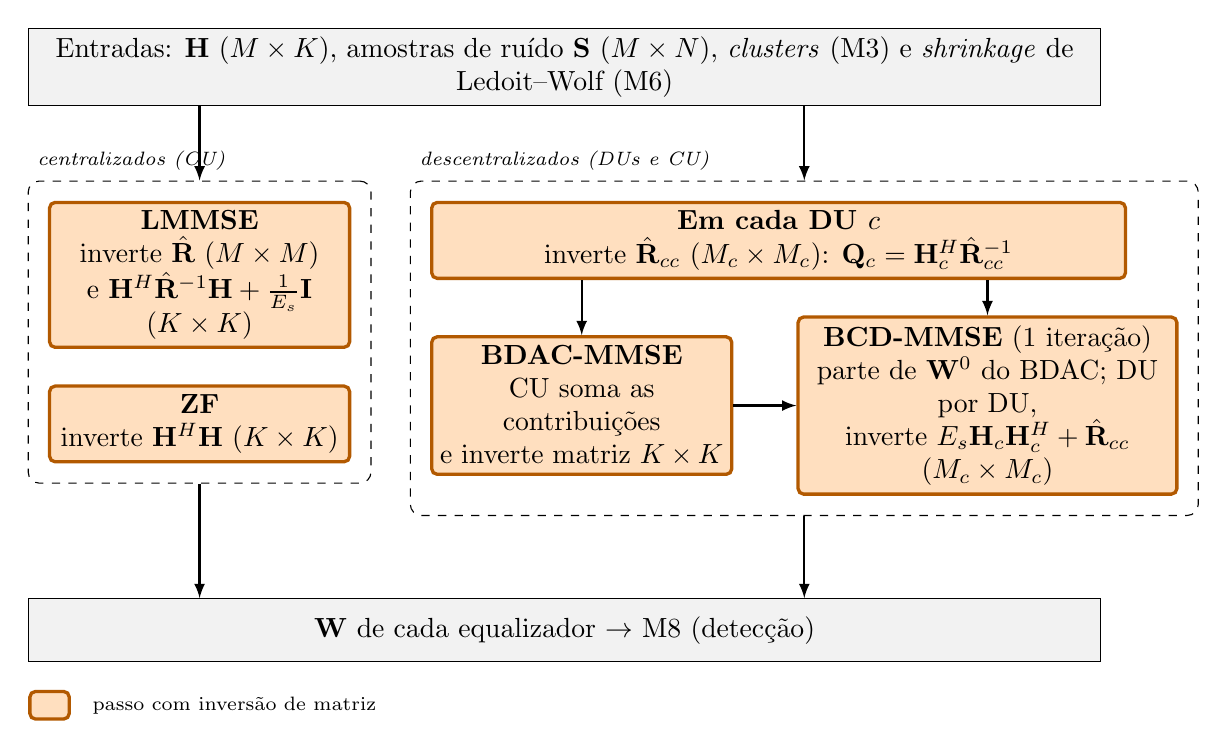
\begin{tikzpicture}[
    node distance = 0.45cm and 0.35cm,
    caixa/.style = {draw, rounded corners=2pt, align=flush center, fill=white,
                     minimum height=0.9cm, inner sep=3pt},
    inv/.style   = {caixa, fill=orange!25, draw=orange!70!black, very thick},
    dado/.style  = {draw, align=flush center, fill=gray!10, minimum height=0.8cm,
                     inner sep=3pt},
    grupo/.style = {draw, dashed, rounded corners=4pt, inner sep=0.25cm},
    seta/.style  = {-latex, thick},
  ]

  % --- entradas -----------------------------------------------------------
  \node[dado, text width=13.4cm] (in) {Entradas: $\mathbf{H}$ ($M \times K$),
    amostras de ruído $\mathbf{S}$ ($M \times N$), \textit{clusters} (M3)
    e \textit{shrinkage} de Ledoit--Wolf (M6)};

  % --- centralizados (CU) -------------------------------------------------
  \node[inv, text width=3.6cm, below=1.2cm of in.south west, anchor=north west,
        xshift=0.25cm] (lmmse) {\textbf{LMMSE}\\
    inverte $\hat{\mathbf{R}}$ ($M \times M$)\\
    e $\mathbf{H}^H\hat{\mathbf{R}}^{-1}\mathbf{H} + \frac{1}{E_s}\mathbf{I}$
    ($K \times K$)};
  \node[inv, text width=3.6cm, below=of lmmse] (zf) {\textbf{ZF}\\
    inverte $\mathbf{H}^H\mathbf{H}$ ($K \times K$)};

  % --- descentralizados ---------------------------------------------------
  \node[inv, text width=8.6cm, right=1.0cm of lmmse.north east, anchor=north west]
    (du) {\textbf{Em cada DU $c$}\\
    inverte $\hat{\mathbf{R}}_{cc}$ ($M_c \times M_c$):
    $\mathbf{Q}_c = \mathbf{H}_c^H\hat{\mathbf{R}}_{cc}^{-1}$};

  \node[inv, text width=3.6cm, below=0.7cm of du.south west, anchor=north west]
    (bdac) {\textbf{BDAC-MMSE}\\ CU soma as contribuições\\ e inverte matriz $K \times K$};
  \node[inv, text width=4.6cm, right=0.8cm of bdac] (bcd) {\textbf{BCD-MMSE} (1 iteração)\\
    parte de $\mathbf{W}^0$ do BDAC; DU por DU,\\
    inverte $E_s\mathbf{H}_c\mathbf{H}_c^H + \hat{\mathbf{R}}_{cc}$
    ($M_c \times M_c$)};

  % --- saída --------------------------------------------------------------
  \node[dado, text width=13.4cm, below=1.3cm of bcd.south -| in] (out)
    {$\mathbf{W}$ de cada equalizador $\rightarrow$ M8 (detecção)};

  % --- grupos -------------------------------------------------------------
  \begin{scope}[on background layer]
    \node[grupo, fit=(lmmse) (zf)] (gcen) {};
    \node[grupo, fit=(du) (bdac) (bcd)] (gdes) {};
  \end{scope}
  \node[anchor=south west, font=\scriptsize\itshape] at (gcen.north west)
    {centralizados (CU)};
  \node[anchor=south west, font=\scriptsize\itshape] at (gdes.north west)
    {descentralizados (DUs e CU)};

  % --- setas --------------------------------------------------------------
  \draw[seta] (in.south -| gcen.north) -- (gcen.north);
  \draw[seta] (in.south -| gdes.north) -- (gdes.north);
  \draw[seta] (du.south -| bdac) -- (bdac);
  \draw[seta] (du.south -| bcd) -- (bcd);
  \draw[seta] (bdac) -- (bcd);
  \draw[seta] (gcen.south) -- (out.north -| gcen.south);
  \draw[seta] (gdes.south) -- (out.north -| gdes.south);

  % --- legenda ------------------------------------------------------------
  \node[inv, minimum height=0.35cm, minimum width=0.5cm, inner sep=0pt,
        below=0.35cm of out.south west, anchor=north west] (leg) {};
  \node[right=0.15cm of leg, font=\scriptsize] {passo com inversão de matriz};
\end{tikzpicture}
\legend{Fonte: a autora.}
\end{figure}
